\documentclass[12pt,a4paper]{article}
\usepackage[utf8]{inputenc}
\usepackage[T1]{fontenc}
\usepackage{lmodern}
\usepackage[margin=1in]{geometry}
\usepackage{amsmath,amssymb}
\usepackage{graphicx}
\usepackage{xcolor}
\usepackage{listings}
\usepackage{booktabs}
\usepackage{enumitem}
\usepackage{tikz}
\usetikzlibrary{shapes,arrows,positioning,calc,fit,backgrounds}
\usepackage{tcolorbox}
\tcbuselibrary{skins,breakable}
\usepackage{fancyhdr}
\usepackage{hyperref}
\usepackage{multicol}
\usepackage{array}
\usepackage{longtable}
\usepackage{caption}

% Colors
\definecolor{codegreen}{rgb}{0,0.6,0}
\definecolor{codegray}{rgb}{0.5,0.5,0.5}
\definecolor{codepurple}{rgb}{0.58,0,0.82}
\definecolor{backcolour}{rgb}{0.95,0.95,0.97}
\definecolor{accentblue}{RGB}{41,98,255}
\definecolor{accentred}{RGB}{220,50,47}
\definecolor{accentgreen}{RGB}{0,150,80}
\definecolor{darkbg}{RGB}{40,44,52}
\definecolor{lightblue}{RGB}{230,240,255}
\definecolor{lightyellow}{RGB}{255,250,230}
\definecolor{lightgreen}{RGB}{230,255,235}
\definecolor{lightred}{RGB}{255,235,235}

% Code listing style
\lstdefinestyle{mystyle}{
    backgroundcolor=\color{backcolour},
    commentstyle=\color{codegreen},
    keywordstyle=\color{accentblue}\bfseries,
    numberstyle=\tiny\color{codegray},
    stringstyle=\color{codepurple},
    basicstyle=\ttfamily\small,
    breakatwhitespace=false,
    breaklines=true,
    captionpos=b,
    keepspaces=true,
    numbers=left,
    numbersep=5pt,
    showspaces=false,
    showstringspaces=false,
    showtabs=false,
    tabsize=2,
    frame=single,
    rulecolor=\color{codegray}
}
\lstset{style=mystyle}

% Box styles
\newtcolorbox{conceptbox}[1]{
    colback=lightblue, colframe=accentblue, fonttitle=\bfseries\large,
    title=#1, breakable, enhanced, sharp corners
}
\newtcolorbox{examplebox}[1]{
    colback=lightgreen, colframe=accentgreen, fonttitle=\bfseries\large,
    title=#1, breakable, enhanced, sharp corners
}
\newtcolorbox{warningbox}[1]{
    colback=lightred, colframe=accentred, fonttitle=\bfseries\large,
    title=#1, breakable, enhanced, sharp corners
}
\newtcolorbox{tipbox}[1]{
    colback=lightyellow, colframe=orange, fonttitle=\bfseries\large,
    title=#1, breakable, enhanced, sharp corners
}

% Header/Footer
\pagestyle{fancy}
\fancyhf{}
\fancyhead[L]{\textbf{Operating System Concepts}}
\fancyhead[R]{\textbf{Interview Guide}}
\fancyfoot[C]{\thepage}
\renewcommand{\headrulewidth}{1pt}

\hypersetup{
    colorlinks=true, linkcolor=accentblue, urlcolor=accentblue, citecolor=accentblue
}

\title{
    \vspace{-1cm}
    {\Huge\textbf{Operating System Concepts}}\\[0.3cm]
    {\LARGE Complete Interview Preparation Guide}\\[0.3cm]
    {\large With Real-World Examples, Diagrams \& Code}
}
\author{}
\date{\today}

\begin{document}
\maketitle
\thispagestyle{fancy}

\tableofcontents
\newpage

% ==============================================================================
\section{Introduction to Operating Systems}
% ==============================================================================

\begin{conceptbox}{What is an Operating System?}
An \textbf{Operating System (OS)} is system software that acts as an intermediary between the user and computer hardware. It manages hardware resources and provides services for application programs.
\end{conceptbox}

\subsection{Functions of an OS}
\begin{center}
\begin{tabular}{@{} l p{6cm} p{4.5cm} @{}}
\toprule
\textbf{Function} & \textbf{Description} & \textbf{Example} \\
\midrule
Process Management & Creates, schedules, terminates processes & Chrome + VS Code running together \\
Memory Management & Allocates/deallocates RAM & Loading a program into memory \\
File Management & Creates, deletes, organizes files & NTFS, ext4 file systems \\
I/O Management & Controls input/output devices & Printer spooling \\
Security & Authentication, access control & Passwords, file permissions \\
\bottomrule
\end{tabular}
\end{center}

\subsection{Types of Operating Systems}
\begin{enumerate}[leftmargin=*]
    \item \textbf{Batch OS} --- Jobs collected in batches, no user interaction (early IBM mainframes).
    \item \textbf{Multiprogramming OS} --- Multiple programs in memory; CPU switches on I/O wait.
    \item \textbf{Multitasking / Time-Sharing} --- CPU time shared using time quantum (UNIX, Linux).
    \item \textbf{Real-Time OS} --- Hard RTOS (missile systems), Soft RTOS (video streaming).
    \item \textbf{Distributed OS} --- Multiple machines work together (Google infrastructure).
\end{enumerate}

\subsection{Kernel Types}
\begin{center}
\begin{tabular}{@{} l p{4cm} l l l @{}}
\toprule
\textbf{Type} & \textbf{Description} & \textbf{Example} & \textbf{Pro} & \textbf{Con} \\
\midrule
Monolithic & All services in kernel space & Linux & Fast & One crash = all crash \\
Microkernel & Minimal kernel; user-space services & QNX & Stable & Slower \\
Hybrid & Mix of both & Windows NT & Balanced & Complex \\
\bottomrule
\end{tabular}
\end{center}

\subsection{User Mode vs Kernel Mode}
\begin{center}
\begin{tabular}{@{} l l l @{}}
\toprule
\textbf{Feature} & \textbf{User Mode} & \textbf{Kernel Mode} \\
\midrule
Privilege & Restricted & Full access \\
Mode bit & 1 & 0 \\
Crash impact & Only that process & Entire system \\
\bottomrule
\end{tabular}
\end{center}
When a process makes a \textbf{system call}, it switches: User Mode $\rightarrow$ Kernel Mode $\rightarrow$ User Mode.

% ==============================================================================
\section{System Calls}
% ==============================================================================

\begin{conceptbox}{Definition}
A \textbf{system call} is a programmatic way for a user process to request a service from the OS kernel. It is the interface between user programs and the operating system.
\end{conceptbox}

\subsection{Categories}

\begin{center}
\begin{tabular}{@{} l l p{7cm} @{}}
\toprule
\textbf{Category} & \textbf{Calls} & \textbf{Description} \\
\midrule
Process Control & \texttt{fork(), exec(), wait(), exit()} & Create, replace, wait, terminate processes \\
File Management & \texttt{open(), read(), write(), close()} & File I/O operations \\
Device Management & \texttt{ioctl(), read(), write()} & Device-specific operations \\
Information & \texttt{getpid(), time(), alarm()} & System/process info \\
Communication & \texttt{pipe(), shmget(), socket()} & IPC and networking \\
\bottomrule
\end{tabular}
\end{center}

\begin{examplebox}{fork() Example}
\begin{lstlisting}[language=C]
#include <stdio.h>
#include <unistd.h>
#include <sys/wait.h>

int main() {
    int pid = fork();
    if (pid == 0) {
        printf("Child PID: %d\n", getpid());
    } else if (pid > 0) {
        printf("Parent PID: %d, Child: %d\n", getpid(), pid);
        wait(NULL);
    } else {
        printf("Fork failed!\n");
    }
    return 0;
}
// Output:
// Parent PID: 1234, Child: 1235
// Child PID: 1235
\end{lstlisting}

\texttt{fork()} returns: \textbf{0} to child, \textbf{child PID} to parent, \textbf{-1} on failure.
\end{examplebox}

% ==============================================================================
\section{Process Management}
% ==============================================================================

\subsection{Process Memory Layout}

\begin{center}
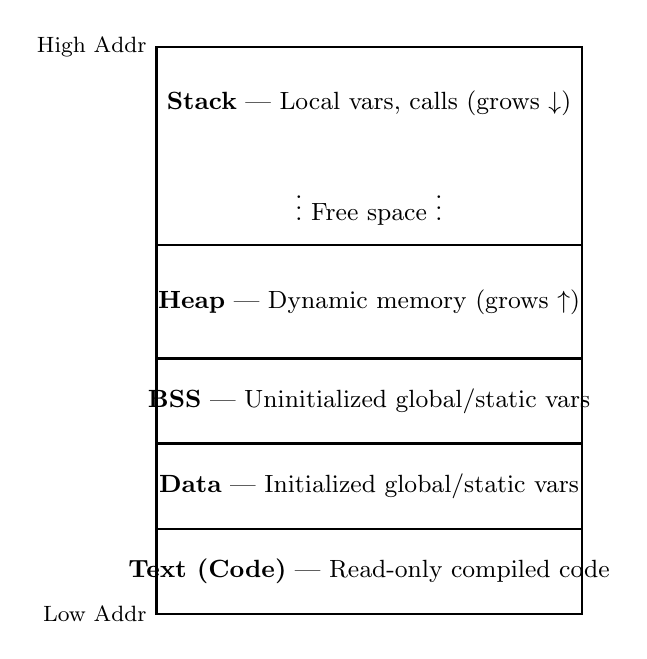
\begin{tikzpicture}[scale=0.9, every node/.style={font=\small}]
    \draw[thick] (0,0) rectangle (6,8);
    \draw[thick] (0,1.2) -- (6,1.2);
    \draw[thick] (0,2.4) -- (6,2.4);
    \draw[thick] (0,3.6) -- (6,3.6);
    \draw[thick] (0,5.2) -- (6,5.2);
    
    \node at (3,0.6) {\textbf{Text (Code)} --- Read-only compiled code};
    \node at (3,1.8) {\textbf{Data} --- Initialized global/static vars};
    \node at (3,3.0) {\textbf{BSS} --- Uninitialized global/static vars};
    \node at (3,4.4) {\textbf{Heap} --- Dynamic memory (grows $\uparrow$)};
    \node at (3,5.8) {$\vdots$ Free space $\vdots$};
    \node at (3,7.2) {\textbf{Stack} --- Local vars, calls (grows $\downarrow$)};
    
    \node[left] at (0,0) {\footnotesize Low Addr};
    \node[left] at (0,8) {\footnotesize High Addr};
\end{tikzpicture}
\end{center}

\subsection{Stack vs Heap}
\begin{center}
\begin{tabular}{@{} l l @{}}
\toprule
\textbf{Stack} & \textbf{Heap} \\
\midrule
Automatic alloc/dealloc & Manual (\texttt{malloc/free}) \\
LIFO, very fast & No order, slower \\
Limited size (1--8 MB) & Limited by available RAM \\
Local variables, return addresses & Dynamically allocated objects \\
\bottomrule
\end{tabular}
\end{center}

\subsection{Process States}

\begin{center}
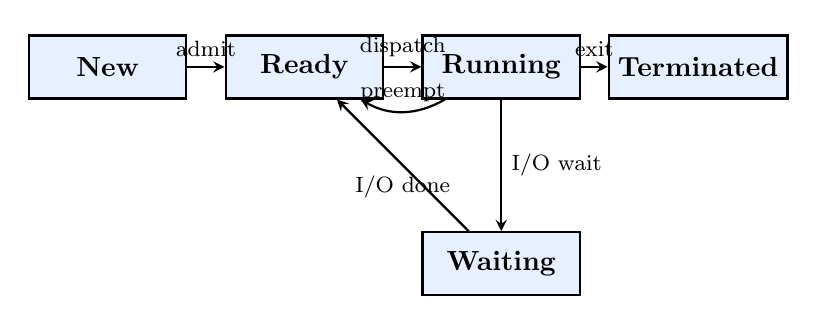
\begin{tikzpicture}[node distance=2.5cm, auto,
    state/.style={rectangle, draw, thick, fill=lightblue, minimum width=2cm, minimum height=0.8cm, font=\bfseries},
    arr/.style={->, thick, >=stealth}]
    
    \node[state] (new) {New};
    \node[state, right of=new] (ready) {Ready};
    \node[state, right of=ready] (running) {Running};
    \node[state, right of=running] (term) {Terminated};
    \node[state, below of=running] (waiting) {Waiting};
    
    \draw[arr] (new) -- node[above]{\footnotesize admit} (ready);
    \draw[arr] (ready) -- node[above]{\footnotesize dispatch} (running);
    \draw[arr] (running) -- node[above]{\footnotesize exit} (term);
    \draw[arr] (running) -- node[right]{\footnotesize I/O wait} (waiting);
    \draw[arr] (waiting) -- node[below]{\footnotesize I/O done} (ready);
    \draw[arr] (running) to[bend left=30] node[above]{\footnotesize preempt} (ready);
\end{tikzpicture}
\end{center}

\subsection{Context Switching}
\textbf{Context switch} = save state of current process into its PCB, load state of next process from its PCB. This is \textbf{pure overhead} (no useful work). Typical time: 1--10 $\mu$s.

\subsection{Zombie vs Orphan Process}
\begin{center}
\begin{tabular}{@{} l p{5.5cm} p{5cm} @{}}
\toprule
& \textbf{Zombie} & \textbf{Orphan} \\
\midrule
Cause & Child terminated, parent didn't \texttt{wait()} & Parent terminated first \\
Fix & Parent calls \texttt{wait()} & Adopted by \texttt{init} (PID 1) \\
\bottomrule
\end{tabular}
\end{center}

\subsection{Inter-Process Communication (IPC)}
\begin{center}
\begin{tabular}{@{} l l l @{}}
\toprule
\textbf{Method} & \textbf{Speed} & \textbf{Sync Needed?} \\
\midrule
Shared Memory & Fast & Yes (semaphores) \\
Message Passing & Slower & No \\
Pipes & Moderate & No \\
Sockets & Network-capable & No \\
Signals & Asynchronous & N/A \\
\bottomrule
\end{tabular}
\end{center}

% ==============================================================================
\section{CPU Scheduling}
% ==============================================================================

\subsection{Scheduling Criteria}
\begin{itemize}[leftmargin=*]
    \item \textbf{CPU Utilization} --- keep CPU busy (40--90\%)
    \item \textbf{Throughput} --- processes completed per unit time
    \item \textbf{Turnaround Time (TAT)} --- submission to completion
    \item \textbf{Waiting Time (WT)} --- time in ready queue
    \item \textbf{Response Time} --- request to first response
\end{itemize}

\subsection{FCFS (First Come First Served) --- Non-preemptive}

\begin{examplebox}{FCFS Example}
\begin{center}
\begin{tabular}{@{} c c c @{}}
\toprule
\textbf{Process} & \textbf{Arrival} & \textbf{Burst} \\
\midrule
P1 & 0 & 24 \\
P2 & 1 & 3 \\
P3 & 2 & 3 \\
\bottomrule
\end{tabular}
\end{center}

\textbf{Gantt Chart:}
\begin{center}
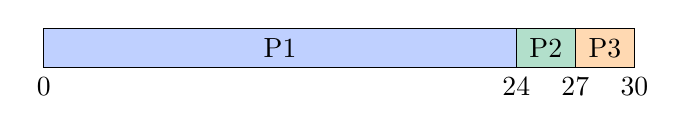
\begin{tikzpicture}[scale=0.5]
    \draw[fill=accentblue!30] (0,0) rectangle (12,1); \node at (6,0.5) {P1};
    \draw[fill=accentgreen!30] (12,0) rectangle (13.5,1); \node at (12.75,0.5) {P2};
    \draw[fill=orange!30] (13.5,0) rectangle (15,1); \node at (14.25,0.5) {P3};
    \node[below] at (0,0) {0}; \node[below] at (12,0) {24}; 
    \node[below] at (13.5,0) {27}; \node[below] at (15,0) {30};
\end{tikzpicture}
\end{center}

\textbf{Calculations:}
\begin{align*}
\text{WT}_{P1} &= 0, \quad \text{WT}_{P2} = 24 - 1 = 23, \quad \text{WT}_{P3} = 27 - 2 = 25 \\
\text{Avg WT} &= \frac{0 + 23 + 25}{3} = \boxed{16.0} \\
\text{TAT}_{P1} &= 24, \quad \text{TAT}_{P2} = 26, \quad \text{TAT}_{P3} = 28 \\
\text{Avg TAT} &= \frac{24 + 26 + 28}{3} = \boxed{26.0}
\end{align*}

\textbf{Problem:} \textcolor{red}{Convoy Effect} --- short processes stuck behind long ones.
\end{examplebox}

\subsection{SJF (Shortest Job First) --- Non-preemptive}
Selects process with smallest burst time. \textbf{Optimal} for avg waiting time.

\textbf{Problem:} \textcolor{red}{Starvation} --- long processes may never get CPU.

\subsection{SRTF (Shortest Remaining Time First) --- Preemptive SJF}
At each new arrival, compare remaining times and preempt if a shorter job arrives.

\subsection{Round Robin --- Preemptive}

\begin{examplebox}{Round Robin Example (q = 4)}
\begin{center}
\begin{tabular}{@{} c c c @{}}
\toprule
\textbf{Process} & \textbf{Arrival} & \textbf{Burst} \\
\midrule
P1 & 0 & 5 \\
P2 & 1 & 3 \\
P3 & 2 & 8 \\
\bottomrule
\end{tabular}
\end{center}

\textbf{Execution:}
\begin{itemize}[leftmargin=*]
    \item $[0, 4)$: P1 runs (remaining = 1)
    \item $[4, 7)$: P2 runs (done, burst = 3)
    \item $[7, 11)$: P3 runs (remaining = 4)
    \item $[11, 12)$: P1 runs (done)
    \item $[12, 16)$: P3 runs (done)
\end{itemize}

Key: If $q$ too large $\rightarrow$ FCFS. If $q$ too small $\rightarrow$ too many context switches. Typical $q$: 10--100 ms.
\end{examplebox}

\subsection{Priority Scheduling}
Highest priority first. \textcolor{red}{Problem: Starvation.} \textcolor{accentgreen}{Solution: Aging.}

\subsection{Multilevel Feedback Queue}
Multiple queues with different time quanta. Processes move between queues (prevents starvation). \textbf{Most general and flexible} algorithm.

% ==============================================================================
\section{Threads \& Multithreading}
% ==============================================================================

\begin{conceptbox}{Thread}
A \textbf{thread} is the smallest unit of CPU execution. A process can have multiple threads sharing the same address space but each with its own stack, registers, and program counter.
\end{conceptbox}

\subsection{Process vs Thread}
\begin{center}
\begin{tabular}{@{} l l l @{}}
\toprule
\textbf{Feature} & \textbf{Process} & \textbf{Thread} \\
\midrule
Memory & Separate address space & Shares process memory \\
Creation time & Slow ($\sim$ms) & Fast ($\sim\mu$s) \\
Communication & IPC needed & Direct shared memory \\
Context switch & Expensive & Cheap \\
Crash impact & Only that process & Entire process crashes \\
\bottomrule
\end{tabular}
\end{center}

\subsection{Threading Models}
\begin{itemize}[leftmargin=*]
    \item \textbf{Many-to-One:} Many user threads $\rightarrow$ 1 kernel thread. No true parallelism.
    \item \textbf{One-to-One:} Each user thread $\rightarrow$ 1 kernel thread (Linux). True parallelism.
    \item \textbf{Many-to-Many:} $M$ user threads $\rightarrow$ $N$ kernel threads. Best of both worlds.
\end{itemize}

% ==============================================================================
\section{Process Synchronization}
% ==============================================================================

\subsection{Race Condition}
\begin{warningbox}{Race Condition Example}
\begin{lstlisting}[language=C]
int counter = 5;
// Thread A: counter++    Thread B: counter--
// Expected: 5. Actual: could be 4, 5, or 6!
\end{lstlisting}
\texttt{counter++} is \textbf{NOT atomic}: LOAD $\rightarrow$ ADD $\rightarrow$ STORE. Interleaving corrupts the result.
\end{warningbox}

\subsection{Critical Section Requirements}
\begin{enumerate}
    \item \textbf{Mutual Exclusion:} Only one process in CS at a time.
    \item \textbf{Progress:} No unnecessary blocking of waiting processes.
    \item \textbf{Bounded Waiting:} A limit on how long a process waits.
\end{enumerate}

\subsection{Mutex \& Semaphore}
\begin{center}
\begin{tabular}{@{} l p{5.5cm} p{5.5cm} @{}}
\toprule
& \textbf{Mutex} & \textbf{Semaphore} \\
\midrule
Type & Binary lock (0/1) & Counter (0 to $N$) \\
Ownership & Owned by locking thread & No ownership \\
Use case & Mutual exclusion & Controlling $N$ resource instances \\
\bottomrule
\end{tabular}
\end{center}

\subsection{Classic Problems}
\begin{examplebox}{Producer-Consumer (Bounded Buffer)}
\begin{lstlisting}[language=C,escapechar=@]
// Semaphores: mutex=1, empty=N, full=0

// Producer:                    // Consumer:
wait(empty);                    wait(full);
wait(mutex);                    wait(mutex);
buffer[in] = item;              item = buffer[out];
in = (in+1) % N;               out = (out+1) % N;
signal(mutex);                  signal(mutex);
signal(full);                   signal(empty);
\end{lstlisting}
\end{examplebox}

\textbf{Readers-Writers:} Multiple readers OR one writer. \\
\textbf{Dining Philosophers:} 5 philosophers, 5 forks. Naive $\rightarrow$ deadlock. Fix: limit to 4 at table or asymmetric pickup.

% ==============================================================================
\section{Deadlocks}
% ==============================================================================

\begin{warningbox}{Four Necessary Conditions (ALL must hold)}
\begin{enumerate}
    \item \textbf{Mutual Exclusion:} Non-sharable resource.
    \item \textbf{Hold and Wait:} Hold one resource, wait for another.
    \item \textbf{No Preemption:} Cannot forcibly take resources.
    \item \textbf{Circular Wait:} $P_1 \rightarrow P_2 \rightarrow P_3 \rightarrow P_1$.
\end{enumerate}
\textbf{Mnemonic: M-H-N-C}
\end{warningbox}

\subsection{Banker's Algorithm (Deadlock Avoidance)}
\begin{examplebox}{Banker's Algorithm --- Full Worked Example}
5 processes ($P_0$--$P_4$), 3 resource types: $A=10, B=5, C=7$.

\begin{center}
\begin{tabular}{@{} c ccc ccc ccc ccc @{}}
\toprule
& \multicolumn{3}{c}{\textbf{Allocation}} & \multicolumn{3}{c}{\textbf{Maximum}} & \multicolumn{3}{c}{\textbf{Need}} & \multicolumn{3}{c}{\textbf{Available}} \\
& A & B & C & A & B & C & A & B & C & A & B & C \\
\midrule
$P_0$ & 0 & 1 & 0 & 7 & 5 & 3 & 7 & 4 & 3 & 3 & 3 & 2 \\
$P_1$ & 2 & 0 & 0 & 3 & 2 & 2 & 1 & 2 & 2 & & & \\
$P_2$ & 3 & 0 & 2 & 9 & 0 & 2 & 6 & 0 & 0 & & & \\
$P_3$ & 2 & 1 & 1 & 2 & 2 & 2 & 0 & 1 & 1 & & & \\
$P_4$ & 0 & 0 & 2 & 4 & 3 & 3 & 4 & 3 & 1 & & & \\
\bottomrule
\end{tabular}
\end{center}

\textbf{Safety Check:}
\begin{enumerate}
    \item Available $=(3,3,2)$. $P_1$: Need$(1,2,2) \leq (3,3,2)$ $\checkmark$ $\Rightarrow$ Available $= (5,3,2)$
    \item $P_3$: Need$(0,1,1) \leq (5,3,2)$ $\checkmark$ $\Rightarrow$ Available $= (7,4,3)$
    \item $P_0$: Need$(7,4,3) \leq (7,4,3)$ $\checkmark$ $\Rightarrow$ Available $= (7,5,3)$
    \item $P_2$: Need$(6,0,0) \leq (7,5,3)$ $\checkmark$ $\Rightarrow$ Available $= (10,5,5)$
    \item $P_4$: Need$(4,3,1) \leq (10,5,5)$ $\checkmark$
\end{enumerate}
\textbf{Safe Sequence:} $\langle P_1, P_3, P_0, P_2, P_4 \rangle$ \quad $\checkmark$ \textbf{SAFE STATE}
\end{examplebox}

% ==============================================================================
\section{Memory Management}
% ==============================================================================

\subsection{Logical vs Physical Address}
\begin{itemize}[leftmargin=*]
    \item \textbf{Logical (Virtual) Address:} Generated by CPU. Used by programmer.
    \item \textbf{Physical Address:} Actual location in RAM.
    \item \textbf{MMU} translates: Physical $=$ Base $+$ Logical.
\end{itemize}

\subsection{Fragmentation}
\begin{center}
\begin{tabular}{@{} l p{5.5cm} p{5.5cm} @{}}
\toprule
& \textbf{Internal} & \textbf{External} \\
\midrule
What & Wasted space \textit{inside} allocated block & Free memory exists but is \textit{not contiguous} \\
Cause & Fixed-size partitioning & Variable-size partitioning \\
Fix & Use smaller partitions / paging & Compaction or paging \\
\bottomrule
\end{tabular}
\end{center}

\subsection{Allocation Strategies}
\begin{itemize}[leftmargin=*]
    \item \textbf{First Fit:} First hole that fits (fastest, generally best).
    \item \textbf{Best Fit:} Smallest sufficient hole (leaves tiny unusable fragments).
    \item \textbf{Worst Fit:} Largest hole (leaves larger remaining holes).
\end{itemize}

% ==============================================================================
\section{Paging --- Detailed with Examples}
% ==============================================================================

\begin{conceptbox}{What is Paging?}
\textbf{Paging} eliminates external fragmentation by dividing:
\begin{itemize}
    \item \textbf{Logical memory} $\rightarrow$ fixed-size \textbf{Pages}
    \item \textbf{Physical memory} $\rightarrow$ fixed-size \textbf{Frames} (same size as pages)
\end{itemize}
Any page can go into any free frame. A \textbf{page table} maps pages to frames.
\end{conceptbox}

\subsection{Address Translation}
\[
\text{Logical Address} = (\underbrace{p}_{\text{page number}}, \underbrace{d}_{\text{offset}})
\]
\[
\text{Physical Address} = (\text{Frame}[p], d)
\]

If page size $= 2^n$ bytes, and address space $= 2^m$ bytes:
\begin{itemize}
    \item Page offset $= n$ bits
    \item Page number $= m - n$ bits
\end{itemize}

\begin{examplebox}{Paging Calculation Example}
\textbf{Given:}
\begin{itemize}
    \item Logical address space = 16 bytes (4 bits), Page size = 4 bytes
    \item Physical memory = 32 bytes (5 bits), Frame size = 4 bytes = $2^2$
\end{itemize}

\textbf{Page table:}
\begin{center}
\begin{tabular}{cc}
\toprule
\textbf{Page} & \textbf{Frame} \\
\midrule
0 & 5 \\
1 & 6 \\
2 & 1 \\
3 & 2 \\
\bottomrule
\end{tabular}
\end{center}

\textbf{Translate logical address 13:}
\begin{align*}
\text{Page number } p &= \lfloor 13 / 4 \rfloor = 3 \\
\text{Offset } d &= 13 \mod 4 = 1 \\
\text{Frame}[3] &= 2 \\
\text{Physical address} &= 2 \times 4 + 1 = \boxed{9}
\end{align*}

\textbf{Translate logical address 4:}
\begin{align*}
p &= \lfloor 4/4 \rfloor = 1, \quad d = 0 \\
\text{Frame}[1] &= 6 \\
\text{Physical address} &= 6 \times 4 + 0 = \boxed{24}
\end{align*}
\end{examplebox}

\subsection{TLB (Translation Lookaside Buffer)}

TLB is a \textbf{fast hardware cache} for the page table.

\begin{examplebox}{Effective Access Time (EAT) Calculation}
\[
\text{EAT} = h \times (t_{\text{TLB}} + t_{\text{mem}}) + (1-h) \times (t_{\text{TLB}} + 2 \times t_{\text{mem}})
\]

\textbf{Given:} TLB access $= 10$ ns, Memory access $= 100$ ns, Hit ratio $= 90\%$
\begin{align*}
\text{EAT} &= 0.9 \times (10 + 100) + 0.1 \times (10 + 200) \\
           &= 0.9 \times 110 + 0.1 \times 210 = 99 + 21 = \boxed{120 \text{ ns}}
\end{align*}
Without TLB: $200$ ns (two memory accesses). TLB gives \textbf{40\% speedup}.
\end{examplebox}

\subsection{Multi-level Page Tables}
For 32-bit address, 4KB pages:
\[
\underbrace{10 \text{ bits}}_{\text{Outer PT}} \; | \; \underbrace{10 \text{ bits}}_{\text{Inner PT}} \; | \; \underbrace{12 \text{ bits}}_{\text{Offset}}
\]

\subsection{Inverted Page Table}
One entry per \textbf{physical frame} (not per logical page). Saves memory. Used in PowerPC.

% ==============================================================================
\section{Segmentation --- Detailed with Examples}
% ==============================================================================

\begin{conceptbox}{What is Segmentation?}
\textbf{Segmentation} divides memory into \textbf{variable-sized segments} based on \textit{logical units}: code, data, stack, heap. Each segment has a \textbf{base} (start address) and \textbf{limit} (length).

\[
\text{Logical Address} = (\text{segment number } s, \text{ offset } d)
\]
\[
\text{Physical Address} = \text{Base}[s] + d \quad \text{(if } d < \text{Limit}[s]\text{)}
\]
If $d \geq \text{Limit}[s]$ $\Rightarrow$ \textbf{Segmentation Fault!}
\end{conceptbox}

\begin{examplebox}{Segmentation Example}
A process has 4 segments:

\begin{center}
\begin{tabular}{@{} c l c c @{}}
\toprule
\textbf{Segment \#} & \textbf{Name} & \textbf{Base} & \textbf{Limit} \\
\midrule
0 & Code & 1000 & 500 \\
1 & Data & 2000 & 200 \\
2 & Stack & 5000 & 300 \\
3 & Heap & 6000 & 400 \\
\bottomrule
\end{tabular}
\end{center}

\textbf{Translate (1, 150):} Segment 1 (Data), offset 150.
\begin{align*}
d = 150 &< \text{Limit}[1] = 200 \quad \checkmark \\
\text{Physical} &= \text{Base}[1] + d = 2000 + 150 = \boxed{2150}
\end{align*}

\textbf{Translate (2, 350):} Segment 2 (Stack), offset 350.
\begin{align*}
d = 350 &\geq \text{Limit}[2] = 300 \quad \Rightarrow \boxed{\text{SEGMENTATION FAULT!}}
\end{align*}

\textbf{Translate (0, 100):} Segment 0 (Code), offset 100.
\begin{align*}
d = 100 &< 500 \quad \checkmark \\
\text{Physical} &= 1000 + 100 = \boxed{1100}
\end{align*}
\end{examplebox}

\subsection{Paging vs Segmentation}
\begin{center}
\begin{tabular}{@{} l p{5.5cm} p{5.5cm} @{}}
\toprule
\textbf{Feature} & \textbf{Paging} & \textbf{Segmentation} \\
\midrule
Size & Fixed-size pages & Variable-size segments \\
Fragmentation & Internal fragmentation & External fragmentation \\
View & OS perspective (invisible to programmer) & Programmer perspective (logical units) \\
Address & (page \#, offset) & (segment \#, offset) \\
Sharing & Harder & Easy (share a segment) \\
\bottomrule
\end{tabular}
\end{center}

\subsection{Segmented Paging (Used in x86)}
Modern systems combine both: each \textbf{segment} is divided into \textbf{pages}.
\[
\text{Address: } (\text{segment}, \text{page}, \text{offset})
\]
Gets benefits of both: logical grouping from segmentation + no external fragmentation from paging.

% ==============================================================================
\section{Virtual Memory}
% ==============================================================================

\begin{conceptbox}{Virtual Memory}
Allows execution of processes \textbf{not completely in memory}. Uses disk (swap space) as extension of RAM. Only needed pages are loaded (\textbf{demand paging}).
\end{conceptbox}

\subsection{Page Fault Handling}
\begin{enumerate}
    \item CPU generates logical address.
    \item Page table check: valid bit $= 0 \Rightarrow$ \textbf{PAGE FAULT} (trap).
    \item OS finds free frame (or runs page replacement).
    \item Reads page from disk into frame.
    \item Updates page table, restarts instruction.
\end{enumerate}

\begin{examplebox}{Demand Paging Performance}
\[
\text{EAT} = (1 - p) \times t_{\text{mem}} + p \times t_{\text{fault}}
\]
\textbf{Given:} $t_{\text{mem}} = 200$ ns, $t_{\text{fault}} = 8$ ms $= 8{,}000{,}000$ ns, $p = 0.001$
\begin{align*}
\text{EAT} &= 0.999 \times 200 + 0.001 \times 8{,}000{,}000 \\
           &= 199.8 + 8000 = \boxed{8199.8 \text{ ns}} \approx 8.2 \;\mu\text{s} \quad \text{(40$\times$ slowdown!)}
\end{align*}
\end{examplebox}

\subsection{Page Replacement Algorithms}

\begin{center}
\begin{tabular}{@{} l l l l @{}}
\toprule
\textbf{Algorithm} & \textbf{Strategy} & \textbf{Belady's Anomaly?} & \textbf{Practical?} \\
\midrule
FIFO & Replace oldest & YES & Simple \\
Optimal & Replace farthest future use & No & No (needs future) \\
LRU & Replace least recently used & No & Expensive to implement \\
Clock & Second chance (reference bit) & No & Efficient \\
\bottomrule
\end{tabular}
\end{center}

\begin{examplebox}{LRU Page Replacement Example}
Reference string: 7, 0, 1, 2, 0, 3, 0, 4. \quad Frames = 3.

\begin{center}
\begin{tabular}{@{} c c c l @{}}
\toprule
\textbf{Ref} & \textbf{Frames (MRU$\rightarrow$LRU)} & \textbf{Fault?} & \textbf{Action} \\
\midrule
7 & \{7\} & $\checkmark$ & Load 7 \\
0 & \{0, 7\} & $\checkmark$ & Load 0 \\
1 & \{1, 0, 7\} & $\checkmark$ & Load 1 \\
2 & \{2, 1, 0\} & $\checkmark$ & Replace 7 (LRU) \\
0 & \{0, 2, 1\} & Hit & Move 0 to front \\
3 & \{3, 0, 2\} & $\checkmark$ & Replace 1 (LRU) \\
0 & \{0, 3, 2\} & Hit & Move 0 to front \\
4 & \{4, 0, 3\} & $\checkmark$ & Replace 2 (LRU) \\
\bottomrule
\end{tabular}
\end{center}
\textbf{Total page faults: 6}
\end{examplebox}

\subsection{Thrashing}
Process spends more time \textbf{paging} than \textbf{executing}.

\textbf{Cause:} Too many processes, not enough frames per process.\\
\textbf{Solutions:} Working Set Model (track recent pages), Page Fault Frequency monitoring, reduce degree of multiprogramming.

% ==============================================================================
\section{File Systems}
% ==============================================================================

\subsection{File Allocation Methods}

\begin{center}
\begin{tabular}{@{} l p{4cm} p{3cm} p{3.5cm} @{}}
\toprule
\textbf{Method} & \textbf{How} & \textbf{Pros} & \textbf{Cons} \\
\midrule
Contiguous & Sequential blocks & Fast access & External frag \\
Linked & Blocks linked via pointers & No frag, growable & Slow random access \\
Indexed & Index block with pointers & Fast random access & Index overhead \\
\bottomrule
\end{tabular}
\end{center}

\subsection{UNIX Inode Structure}
\begin{itemize}[leftmargin=*]
    \item 12 \textbf{direct} block pointers
    \item 1 \textbf{single indirect} (pointer to block of pointers)
    \item 1 \textbf{double indirect}
    \item 1 \textbf{triple indirect}
\end{itemize}

Max file size with 4KB blocks, 4-byte pointers:
\[
\text{Direct: } 12 \times 4\text{KB} = 48\text{KB}, \quad \text{Single: } 1024 \times 4\text{KB} = 4\text{MB}
\]
\[
\text{Double: } 1024^2 \times 4\text{KB} = 4\text{GB}, \quad \text{Triple: } 1024^3 \times 4\text{KB} \approx 4\text{TB}
\]

\subsection{Hard Link vs Soft Link}
\begin{center}
\begin{tabular}{@{} l l l @{}}
\toprule
& \textbf{Hard Link} & \textbf{Soft Link} \\
\midrule
Points to & Same inode & Target path \\
Cross filesystem & No & Yes \\
Delete original & Still works & Dangling link \\
\bottomrule
\end{tabular}
\end{center}

% ==============================================================================
\section{Disk Scheduling}
% ==============================================================================

\textbf{Disk Access Time} $=$ Seek Time $+$ Rotational Latency $+$ Transfer Time.

\begin{examplebox}{Disk Scheduling Comparison}
Head at track 53, queue: 98, 183, 37, 122, 14, 124, 65, 67.

\begin{center}
\begin{tabular}{@{} l c c l @{}}
\toprule
\textbf{Algorithm} & \textbf{Total Seek} & \textbf{Starvation?} & \textbf{Notes} \\
\midrule
FCFS & 640 & No & Simple, high seek \\
SSTF & 236 & Yes & Greedy, good avg \\
SCAN & $\sim$236 & No & Elevator \\
C-SCAN & $\sim$382 & No & Uniform wait \\
LOOK & Best & No & Practical default \\
\bottomrule
\end{tabular}
\end{center}
\end{examplebox}

% ==============================================================================
\section{I/O Management}
% ==============================================================================

\begin{center}
\begin{tabular}{@{} l p{6cm} l @{}}
\toprule
\textbf{Method} & \textbf{Description} & \textbf{CPU Usage} \\
\midrule
Polling & CPU repeatedly checks device status & Wastes CPU \\
Interrupt-driven & Device signals CPU when ready & Better \\
DMA & Device transfers directly to memory & Best \\
\bottomrule
\end{tabular}
\end{center}

\textbf{Spooling:} Buffering for slow devices (e.g., printer). Jobs queued to disk, processed later.

% ==============================================================================
\newpage
\section{Real-World Case Study: Google Chrome Browser}
% ==============================================================================

\begin{conceptbox}{How an OS Manages a Web Browser --- End-to-End Example}
This case study traces what happens when you open Google Chrome and browse the web, showing how \textbf{every major OS concept} comes into play.
\end{conceptbox}

\subsection{Step 1: Launching Chrome --- Process Creation}

When you double-click Chrome, the OS performs:

\begin{enumerate}[leftmargin=*]
    \item \textbf{fork()} --- The shell (explorer.exe / bash) creates a child process.
    \item \textbf{exec()} --- The child's memory is replaced with Chrome's binary code.
    \item \textbf{PCB created} --- The OS creates a Process Control Block:
    \begin{itemize}
        \item PID = 5001
        \item State = Ready
        \item Priority = Normal
    \end{itemize}
    \item \textbf{Memory Layout} created:
    \begin{itemize}
        \item \textbf{Text}: Chrome's compiled C++ code ($\sim$150 MB)
        \item \textbf{Data}: Global settings, config variables
        \item \textbf{Heap}: Will grow as you open tabs (DOM trees, images)
        \item \textbf{Stack}: Function call chain
    \end{itemize}
\end{enumerate}

\subsection{Step 2: Opening Tabs --- Multiprocess Architecture}

Chrome uses a \textbf{multi-process model}. Each tab is a separate process:

\begin{center}
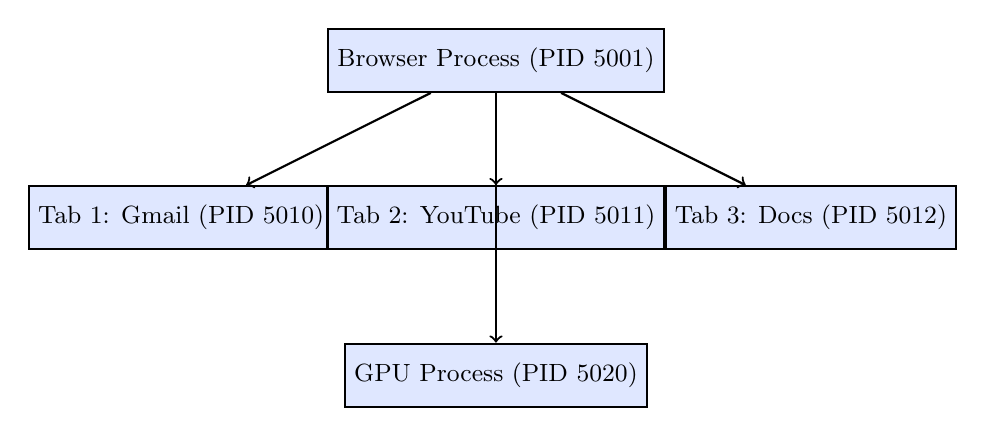
\begin{tikzpicture}[
    proc/.style={rectangle, draw, thick, fill=accentblue!15, minimum width=3.2cm, minimum height=0.8cm, font=\small},
    thread/.style={rectangle, draw, thick, fill=orange!20, minimum width=2.2cm, minimum height=0.6cm, font=\footnotesize}
]
    \node[proc] (browser) at (0,0) {Browser Process (PID 5001)};
    \node[proc] (tab1) at (-4,-2) {Tab 1: Gmail (PID 5010)};
    \node[proc] (tab2) at (0,-2) {Tab 2: YouTube (PID 5011)};
    \node[proc] (tab3) at (4,-2) {Tab 3: Docs (PID 5012)};
    \node[proc] (gpu) at (0,-4) {GPU Process (PID 5020)};
    
    \draw[->, thick] (browser) -- (tab1);
    \draw[->, thick] (browser) -- (tab2);
    \draw[->, thick] (browser) -- (tab3);
    \draw[->, thick] (browser) -- (gpu);
\end{tikzpicture}
\end{center}

\textbf{Why separate processes per tab?}
\begin{itemize}[leftmargin=*]
    \item \textbf{Isolation:} If YouTube tab crashes, Gmail tab survives.
    \item \textbf{Security:} Malicious website in one tab can't access another tab's memory.
    \item \textbf{OS manages each independently} --- separate PCB, separate address space.
\end{itemize}

If Chrome used a single process (like old browsers), one bad tab would crash everything --- this is why \textbf{process isolation} matters.

\subsection{Step 3: Inside a Tab --- Threads}

Each tab process internally uses \textbf{multiple threads}:

\begin{center}
\begin{tabular}{@{} l p{8cm} @{}}
\toprule
\textbf{Thread} & \textbf{Role} \\
\midrule
Main Thread & Runs JavaScript, handles DOM updates \\
Render Thread & Paints pixels to screen (layout, compositing) \\
Network Thread & Fetches resources (HTTP requests) \\
I/O Thread & Reads/writes to disk (cache, downloads) \\
Worker Threads & Background tasks (service workers, Web Workers) \\
\bottomrule
\end{tabular}
\end{center}

\textbf{What threads share:}
\begin{itemize}[leftmargin=*]
    \item Same \textbf{code segment} (Chrome's V8 engine code)
    \item Same \textbf{data segment} (DOM tree, CSS styles)
    \item Same \textbf{heap} (JavaScript objects)
\end{itemize}

\textbf{What each thread has separately:}
\begin{itemize}[leftmargin=*]
    \item Own \textbf{stack} (function call chain)
    \item Own \textbf{registers} and \textbf{program counter}
\end{itemize}

\begin{tipbox}{Interview Connection}
\textit{``Why does Chrome use processes for tabs but threads within a tab?''} \\
\textbf{Answer:} Processes give \textbf{isolation and security} between tabs (crash protection). Threads within a tab give \textbf{performance} (shared memory, fast communication) for rendering, networking, and JavaScript execution that must work together tightly.
\end{tipbox}

\subsection{Step 4: CPU Scheduling in Action}

Your system is running: Chrome (3 tabs), VS Code, Spotify, and OS services.

The \textbf{scheduler} decides who gets the CPU using \textbf{Multilevel Feedback Queue}:

\begin{center}
\begin{tabular}{@{} l l l @{}}
\toprule
\textbf{Queue} & \textbf{Priority} & \textbf{Processes} \\
\midrule
Queue 0 (q=8ms) & Highest & Keyboard/mouse interrupt handlers \\
Queue 1 (q=16ms) & High & Chrome's active tab (foreground) \\
Queue 2 (q=32ms) & Medium & VS Code, Spotify \\
Queue 3 (FCFS) & Low & Background updates, indexing \\
\bottomrule
\end{tabular}
\end{center}

\textbf{What happens when you type in Chrome:}
\begin{enumerate}[leftmargin=*]
    \item Keyboard generates \textbf{hardware interrupt} $\rightarrow$ OS switches to kernel mode.
    \item Interrupt handler (Queue 0) processes the keystroke.
    \item Chrome's main thread (Queue 1) gets scheduled $\rightarrow$ updates the search bar.
    \item Spotify (Queue 2) is \textbf{preempted} briefly but resumes quickly (you don't notice).
    \item A Windows Update download (Queue 3) gets the least CPU time.
\end{enumerate}

\subsection{Step 5: Memory --- Paging \& Frames in Action}

Your PC has \textbf{8 GB RAM} with \textbf{4 KB page/frame size}:
\[
\text{Total frames} = \frac{8 \text{ GB}}{4 \text{ KB}} = \frac{8 \times 1024 \times 1024 \text{ KB}}{4 \text{ KB}} = 2{,}097{,}152 \text{ frames}
\]

Chrome's YouTube tab (PID 5011) uses $\sim$500 MB:
\[
\text{Pages needed} = \frac{500 \text{ MB}}{4 \text{ KB}} = 128{,}000 \text{ pages}
\]

\textbf{How paging works for this tab:}

\begin{center}
\begin{tabular}{@{} l l l l @{}}
\toprule
\textbf{Page} & \textbf{Content} & \textbf{Frame} & \textbf{In RAM?} \\
\midrule
Page 0 & V8 engine code start & Frame 45,201 & Yes \\
Page 1 & V8 engine code cont. & Frame 102,887 & Yes \\
Page 500 & YouTube HTML DOM & Frame 8,442 & Yes \\
Page 800 & Cached video buffer & Frame 200,105 & Yes \\
Page 1200 & Old tab content & --- & \textbf{No (on disk)} \\
Page 5000 & Unused heap space & --- & \textbf{No (not loaded)} \\
\bottomrule
\end{tabular}
\end{center}

\textbf{Key insight:} Pages are \textbf{not contiguous} in physical memory! Page 0 is in frame 45,201 and Page 1 is in frame 102,887. The page table handles this mapping transparently.

\begin{examplebox}{Page Fault Scenario}
You scroll down on YouTube and the browser needs to render a new section of the page stored in Page 1200 (currently on disk).

\begin{enumerate}
    \item CPU tries to access Page 1200 $\rightarrow$ page table says valid bit = 0.
    \item \textbf{PAGE FAULT!} CPU traps to OS.
    \item OS finds a free frame (say Frame 77,543).
    \item OS reads Page 1200 from \textbf{swap space on SSD} into Frame 77,543.
    \item Page table updated: Page 1200 $\rightarrow$ Frame 77,543, valid = 1.
    \item Instruction restarted $\rightarrow$ content renders.
    \item \textbf{Time cost:} $\sim$8 ms (SSD) vs 200 ns (RAM) = \textbf{40,000$\times$ slower!}
\end{enumerate}
\end{examplebox}

\subsection{Step 6: Segmentation in Action}

The YouTube tab's virtual memory is logically divided into segments:

\begin{center}
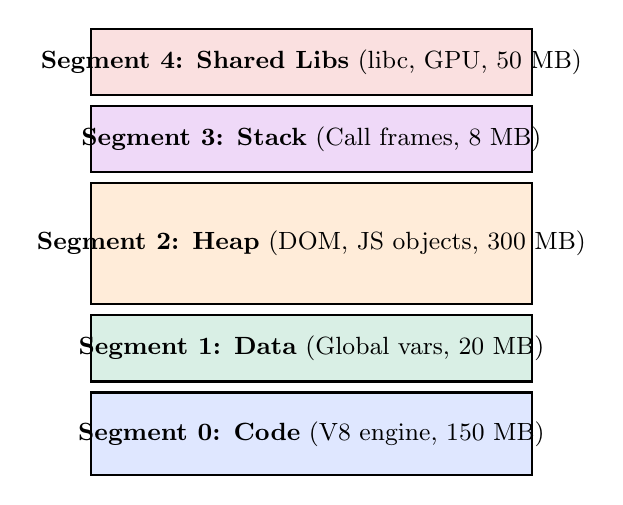
\begin{tikzpicture}[scale=0.7, every node/.style={font=\small}]
    \draw[thick, fill=accentblue!15] (0,0) rectangle (8,1.5);
    \node at (4,0.75) {\textbf{Segment 0: Code} (V8 engine, 150 MB)};
    
    \draw[thick, fill=accentgreen!15] (0,1.7) rectangle (8,2.9);
    \node at (4,2.3) {\textbf{Segment 1: Data} (Global vars, 20 MB)};
    
    \draw[thick, fill=orange!15] (0,3.1) rectangle (8,5.3);
    \node at (4,4.2) {\textbf{Segment 2: Heap} (DOM, JS objects, 300 MB)};
    
    \draw[thick, fill=codepurple!15] (0,5.5) rectangle (8,6.7);
    \node at (4,6.1) {\textbf{Segment 3: Stack} (Call frames, 8 MB)};
    
    \draw[thick, fill=accentred!15] (0,6.9) rectangle (8,8.1);
    \node at (4,7.5) {\textbf{Segment 4: Shared Libs} (libc, GPU, 50 MB)};
\end{tikzpicture}
\end{center}

\textbf{Segment Table:}
\begin{center}
\begin{tabular}{@{} c l c c @{}}
\toprule
\textbf{Seg \#} & \textbf{Name} & \textbf{Base (Physical)} & \textbf{Limit} \\
\midrule
0 & Code & 0x00400000 & 150 MB \\
1 & Data & 0x10000000 & 20 MB \\
2 & Heap & 0x20000000 & 300 MB (grows) \\
3 & Stack & 0x7FFE0000 & 8 MB (grows down) \\
4 & Shared Libs & 0x7F000000 & 50 MB \\
\bottomrule
\end{tabular}
\end{center}

\textbf{What segmentation enables:}
\begin{itemize}[leftmargin=*]
    \item \textbf{Code segment} is \textbf{read-only + shared}. If you open YouTube in 3 tabs, the V8 engine code segment is loaded \textit{once} in RAM and shared across all 3 processes (saving 300 MB!).
    \item \textbf{Stack overflow detection:} If a recursive function exceeds 8 MB, offset $\geq$ limit $\Rightarrow$ \textbf{Segmentation Fault} (the famous ``stack overflow'' error).
    \item \textbf{Heap grows dynamically:} When JavaScript creates objects, the OS expands Segment 2's limit via \texttt{brk()} / \texttt{mmap()} system calls.
\end{itemize}

\begin{warningbox}{Segmentation Fault --- Real Example}
A C program dereferences a NULL pointer:
\begin{lstlisting}[language=C]
int *ptr = NULL;
*ptr = 42;  // Access address 0x00000000
\end{lstlisting}
Address 0x0 belongs to no valid segment $\Rightarrow$ OS generates \textbf{SIGSEGV} (signal 11) $\Rightarrow$ process is \textbf{killed} and you see: \texttt{Segmentation fault (core dumped)}.
\end{warningbox}

\subsection{Step 7: Synchronization Needed}

When the Network Thread downloads a video chunk and the Render Thread needs to display it:

\begin{lstlisting}[language=C]
// Shared buffer between network and render threads
pthread_mutex_t buffer_lock;
sem_t data_available;  // counting semaphore

// Network Thread (Producer):
void* network_thread(void* arg) {
    while (downloading) {
        chunk = download_video_chunk();
        pthread_mutex_lock(&buffer_lock);    // Lock shared buffer
        add_to_buffer(chunk);
        pthread_mutex_unlock(&buffer_lock);  // Unlock
        sem_post(&data_available);           // Signal: data ready
    }
}

// Render Thread (Consumer):
void* render_thread(void* arg) {
    while (playing) {
        sem_wait(&data_available);           // Wait for data
        pthread_mutex_lock(&buffer_lock);
        chunk = get_from_buffer();
        pthread_mutex_unlock(&buffer_lock);
        render_frame(chunk);
    }
}
\end{lstlisting}

This is exactly the \textbf{Producer-Consumer problem} from theory!

\subsection{Step 8: Potential Deadlock Scenario}

Imagine Chrome's tab process needs two resources:
\begin{itemize}[leftmargin=*]
    \item \textbf{Resource A:} GPU memory buffer
    \item \textbf{Resource B:} Network socket
\end{itemize}

\begin{center}
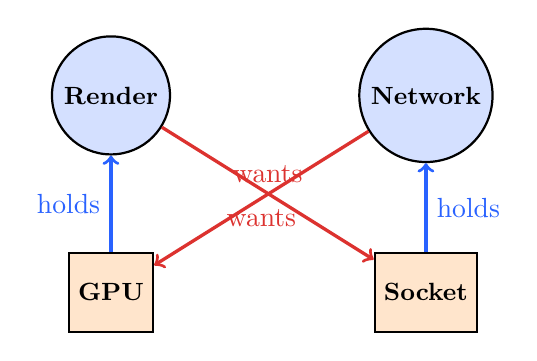
\begin{tikzpicture}[
    proc/.style={circle, draw, thick, fill=accentblue!20, minimum size=1.2cm, font=\small\bfseries},
    res/.style={rectangle, draw, thick, fill=orange!20, minimum size=1cm, font=\small\bfseries}
]
    \node[proc] (p1) at (0,0) {Render};
    \node[proc] (p2) at (4,0) {Network};
    \node[res] (r1) at (0,-2.5) {GPU};
    \node[res] (r2) at (4,-2.5) {Socket};
    
    \draw[->, very thick, accentblue] (r1) -- (p1) node[midway, left] {holds};
    \draw[->, very thick, accentred] (p1) -- (r2) node[midway, above] {wants};
    \draw[->, very thick, accentblue] (r2) -- (p2) node[midway, right] {holds};
    \draw[->, very thick, accentred] (p2) -- (r1) node[midway, below] {wants};
\end{tikzpicture}
\end{center}

\textbf{Circular wait $\Rightarrow$ DEADLOCK!} Chrome avoids this by:
\begin{itemize}[leftmargin=*]
    \item \textbf{Resource ordering:} Always acquire GPU before Socket.
    \item \textbf{Timeouts:} If lock not acquired in 5 seconds, release all and retry.
\end{itemize}

\subsection{Step 9: Virtual Memory \& Thrashing}

You have 50 Chrome tabs open but only 8 GB RAM:

\begin{center}
\begin{tabular}{@{} l c c @{}}
\toprule
\textbf{Process} & \textbf{Virtual Memory} & \textbf{Physical RAM Used} \\
\midrule
Chrome Tab 1--10 (active) & 5 GB & 3 GB \\
Chrome Tab 11--50 (background) & 20 GB & 1 GB (most pages swapped) \\
VS Code & 2 GB & 800 MB \\
Spotify & 500 MB & 200 MB \\
OS + Services & 3 GB & 2 GB \\
\midrule
\textbf{Total} & \textbf{30.5 GB} & \textbf{7 GB (+ 1 GB free)} \\
\bottomrule
\end{tabular}
\end{center}

If you now switch to Tab 35 (which has been swapped to disk):
\begin{enumerate}[leftmargin=*]
    \item Massive page faults as Tab 35's pages are loaded from disk.
    \item To make room, OS \textbf{evicts} pages from other tabs using \textbf{LRU}.
    \item If you keep switching tabs rapidly $\Rightarrow$ \textbf{THRASHING}.
    \item OS detects via \textbf{Page Fault Frequency} and may \textbf{suspend background tabs}.
\end{enumerate}

This is why Chrome shows ``Aw, Snap!'' when tabs run out of memory, and why your PC feels slow with too many tabs!

\subsection{Complete Flow Summary}

\begin{center}
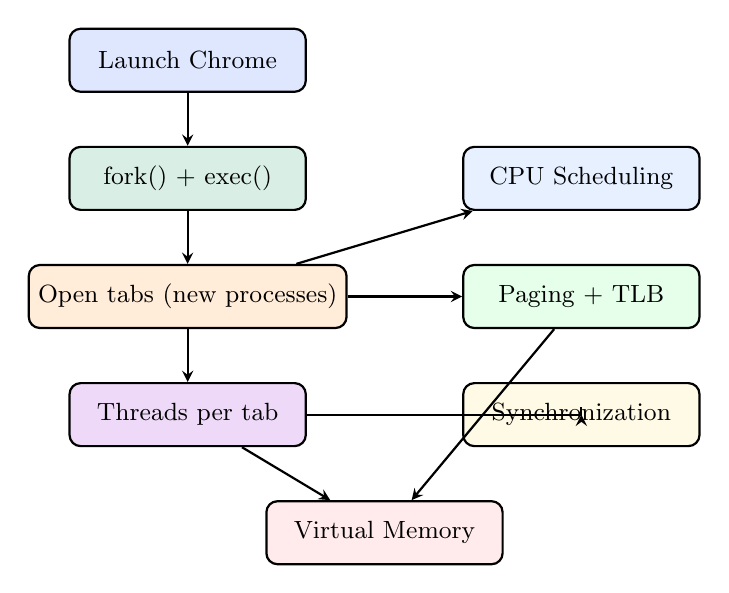
\begin{tikzpicture}[
    box/.style={rectangle, draw, thick, rounded corners, minimum width=3cm, minimum height=0.8cm, font=\small},
    arr/.style={->, thick, >=stealth}
]
    \node[box, fill=accentblue!15] (launch) at (0,0) {Launch Chrome};
    \node[box, fill=accentgreen!15] (fork) at (0,-1.5) {fork() + exec()};
    \node[box, fill=orange!15] (tabs) at (0,-3) {Open tabs (new processes)};
    \node[box, fill=codepurple!15] (threads) at (0,-4.5) {Threads per tab};
    \node[box, fill=lightblue] (sched) at (5,-1.5) {CPU Scheduling};
    \node[box, fill=lightgreen] (paging) at (5,-3) {Paging + TLB};
    \node[box, fill=lightyellow] (sync) at (5,-4.5) {Synchronization};
    \node[box, fill=lightred] (vm) at (2.5,-6) {Virtual Memory};
    
    \draw[arr] (launch) -- (fork);
    \draw[arr] (fork) -- (tabs);
    \draw[arr] (tabs) -- (threads);
    \draw[arr] (threads) -| (sync);
    \draw[arr] (tabs) -- (sched);
    \draw[arr] (tabs) -- (paging);
    \draw[arr] (threads) -- (vm);
    \draw[arr] (paging) -- (vm);
\end{tikzpicture}
\end{center}

% ==============================================================================
\newpage
\section{Important Interview Questions}
% ==============================================================================

\begin{enumerate}[leftmargin=*, label=\textbf{Q\arabic*.}]

\item \textbf{Process vs Thread?} \\
Process: separate memory space, expensive. Thread: shares memory, lightweight. Crash in thread kills entire process.

\item \textbf{What is a deadlock? How to prevent?} \\
All 4 conditions (M-H-N-C) must hold. Break any one, e.g., resource ordering for circular wait.

\item \textbf{What is virtual memory?} \\
Allows processes larger than RAM using disk as extension. Uses demand paging.

\item \textbf{Explain thrashing.} \\
Too many processes $\rightarrow$ not enough frames $\rightarrow$ excessive page faults $\rightarrow$ CPU utilization drops. Fix: reduce multiprogramming, use working set model.

\item \textbf{Paging vs Segmentation?} \\
Paging: fixed-size, no external frag, OS-level. Segmentation: variable-size, logical grouping, programmer-visible.

\item \textbf{Semaphore vs Mutex?} \\
Mutex: binary, owned by thread. Semaphore: counter, no ownership, allows $N$ threads.

\item \textbf{Banker's Algorithm?} \\
Deadlock avoidance. Before granting resource, check if system stays in safe state.

\item \textbf{What is a page fault?} \\
Accessing a page not in RAM triggers trap. OS loads from disk, updates page table, restarts instruction.

\item \textbf{Internal vs External fragmentation?} \\
Internal: wasted space inside block. External: total free space enough but not contiguous.

\item \textbf{Explain fork().} \\
Creates child (copy of parent). Returns 0 to child, PID to parent. Uses Copy-on-Write.

\item \textbf{What is starvation? Solution?} \\
Low-priority process never gets CPU. Fix: \textbf{Aging} (gradually increase priority).

\item \textbf{What is DMA?} \\
Direct Memory Access. Device transfers to/from memory without CPU. CPU only initiates and gets interrupted on completion.

\item \textbf{Explain RAID levels.} \\
RAID 0: striping. RAID 1: mirroring. RAID 5: striping + distributed parity. RAID 10: mirror + stripe.

\item \textbf{What is Belady's Anomaly?} \\
In FIFO, more frames can cause more page faults. Does NOT occur in LRU or Optimal.

\item \textbf{Zombie vs Orphan process?} \\
Zombie: child done, parent didn't \texttt{wait()}. Orphan: parent died, adopted by init.

\item \textbf{Explain Copy-on-Write (COW).} \\
After \texttt{fork()}, parent and child share same pages. Only on write, the page is copied. Saves memory.

\item \textbf{What is a context switch?} \\
Save current process state to PCB, load next process state. Pure overhead, 1--10 $\mu$s.

\item \textbf{Why does Chrome use multiple processes?} \\
Isolation (one tab crash doesn't kill others), security (sandboxing), and independent resource management.

\item \textbf{Explain TLB.} \\
Translation Lookaside Buffer: hardware cache for page table. Avoids double memory access. Hit ratio $>95\%$ typical.

\item \textbf{How does the OS handle a stack overflow?} \\
Stack grows beyond segment limit $\Rightarrow$ segmentation fault (SIGSEGV). OS kills the process.

\end{enumerate}

% ==============================================================================
\section*{Quick Reference Formulas}

\begin{tcolorbox}[colback=lightyellow, colframe=orange, title=\textbf{Important Formulas}]
\begin{align*}
\text{EAT (with TLB)} &= h(t_{\text{TLB}} + t_m) + (1-h)(t_{\text{TLB}} + 2t_m) \\[6pt]
\text{EAT (with paging)} &= (1-p) \cdot t_m + p \cdot t_{\text{fault}} \\[6pt]
\text{Page number} &= \lfloor \text{logical address} / \text{page size} \rfloor \\[4pt]
\text{Offset} &= \text{logical address} \mod \text{page size} \\[4pt]
\text{Physical address} &= \text{frame number} \times \text{frame size} + \text{offset} \\[6pt]
\text{Number of pages} &= \lceil \text{logical address space} / \text{page size} \rceil \\[4pt]
\text{Number of frames} &= \text{physical memory} / \text{frame size} \\[6pt]
\text{Turnaround Time} &= \text{Completion Time} - \text{Arrival Time} \\[4pt]
\text{Waiting Time} &= \text{Turnaround Time} - \text{Burst Time} \\[4pt]
\text{Disk Access Time} &= \text{Seek} + \text{Rotational Latency} + \text{Transfer}
\end{align*}
\end{tcolorbox}

\vfill
\begin{center}
\textit{Prepared for interview preparation. Good luck!}
\end{center}

\end{document}
